\section{Grenzen selbststeuernder produktionslogistischer Prozesse}
\label{sec:Grenzen}

Im vorherigen Kapitel wurden die erarbeiteten Möglichkeiten der
selbststeuernden Prozesse aus dem Beispiel einem vergleichbaren Prozess der
Fließfertigung gegenübergestellt. Hieraus ergeben sich Vorteile von
selbststeuernden Prozessen. Im Folgeden wollen wir veranschaulichen,
das selbststeuernde Prozesse aber auch ihre Grenzen haben.

Die Grenzbetrachtung basiert auf der Darstellung aus \citet{evolution2007}.
In die dort beschriebene Grenzbetrachtung werden die beiden zuvor 
betrachteten Prozesse integriert und die Grenzen von selbsteuernden 
Prozessen werden daraus abgeleitet. Eine Darstellung dieser Grenzbetrachtung
mit der Einordnung des beschriebenen selbststeuernden und klassischen Prozesses
zeigt die folgende \abbildung{Grenzbetrachtung}:

\begin{figure}[htb] 
\centering
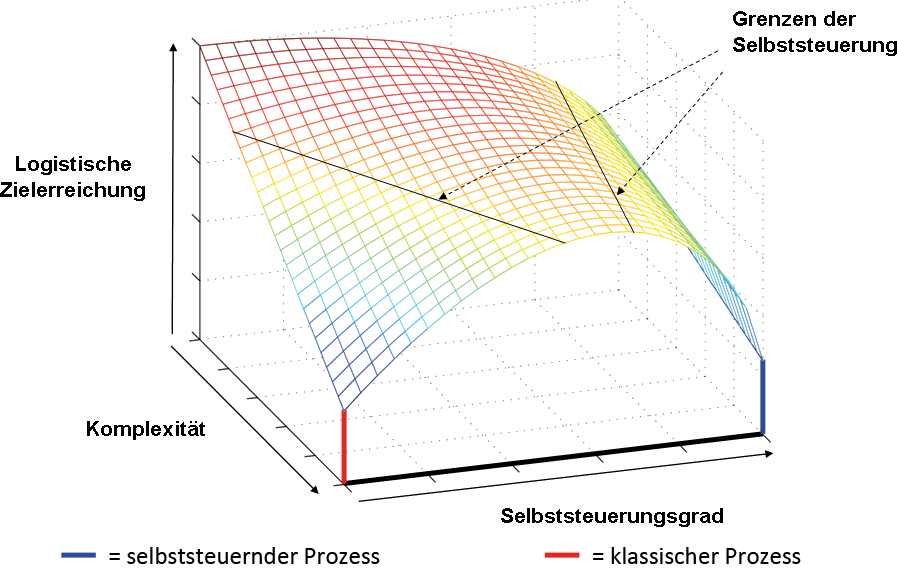
\includegraphics[width=1.0\textwidth]{Grenzbetrachtung.png}
\caption[Grenzbetrachtung]{Grenzen selbststeuernder Prozesse\protect\footnotemark}
\label{fig:Grenzbetrachtung}
\end{figure}
\footnotetext{in Anlehnung an \citet[S.~3]{evolution2007}}

Hierbei gilt es von Anfang an zu verdeutlichen, dass in der dargestellten
Grenzbetrachtung die Grenzen anhand einer "`logistischen Zielerreichung"'
festgelegt wurden. Diese Logistische Zielerreichung setzt sich dabei zusammen
aus mehreren gewichteten Produktionslogistischen Kennzahlen wie zum Beispiel
hohe Termintreue, mittlere Durchlaufzeiten, Bestände und Auslastung.\footnote{Vgl. \citet[S.~4]{evolution2007}}
Diese Logistische Zielerreichung entspricht dabei nicht den Kriterien,
die für den vorherrigen Verlgeich herangezogen wurden.

Aus der dargestellten Abbildung haben wir zwei Grenzen von selbststeuernden Prozesses
im Hinblick auf ihre logistische Zielerreichung herausgearbeitet.

Zunächst kann in der Abbildung gesehen werden, dass die logistische Zielerreichung
des selbststeuernden Prozesses bei der dargestellten Komplexität sehr gering ist.
Diese geringe Zielerreichung können wir begründen mit dem Fehlen von zentralen 
Eingriffs- und Kontrollmöglichkeiten. Dazu ist zu sehen, dass der Selbststeuerungsgrad
des selbststeuernden Prozess in der obigen Abbildung bei 100\% liegt. Aufgrund 
dieser vollständigen Autonomie kann auf eintretende Produktionsfehler nur mit zwei
Möglichkeiten reagiert werden:

\begin{enumerate}
  \item Maschine(n) neu programmieren (Zeitaufwand)
  \item Maschine(n) abschalten (Kostenaufwand)
\end{enumerate}

Beide Möglichkeiten sind dabei aus produktionslogistischer Sicht nicht wünschenswert.
Wir folgern daraus, dass Selbststeuerung immer zentrale Eingriffs- und Kontrollmöglichkeiten
benötigt und vollständige Produktionsautonomie nicht das Ziel sein kann. Dieser \textbf{Kontrollverlust
bei vollständiger Selbststeuerung} ist die erste Grenze selbststeuernder Prozesse
die wir erarbeiten konnten.

Dieser geringen Zielerreichung des selbststeuernden Prozesses steht ein relativ
hoher Grad der Zielerreichung beim klassischen Prozesses gegenüber.
Diese Diskrepanz der Zielerreichung führen wir auf die geringe
Komplexität des betrachteten Produktionsprozesses zurück.
Der betrachtete Produktionsprozess der Rücklichterfertigung besteht nur aus
drei verschiedenen Varianten und vier Fertigungsmaschinen und ist aus diesem
Grund mit dargestellter geringer Komplexität eingeordnet. Diese geringe
Komplexität ermöglicht es, dass der klassische Prozesse effektiv über ein zentrales
System ohne Selbststeuerung gesteuert werden kann (in unserm Beispiel wäre dies der Produktionsplan).
Bei dieser geringen Komplexität fehlt der Bedarf nach Selbststeuerung bzw. autonomer Entscheidungsfindung,
da auch ohne diese die produktionslogistischen Ziele erreicht werden können.
Weiterhin spart man beim Einsatz eines klassischen Prozesses die Kosten für 
die Implementierung einer Selbststeuerung und es wird kein zusätzliches 
Know-How benötigt. Die Grenze die wir hier feststellen ist der \textbf{fehlende Mehrwert}
selbststeuernder Prozesse \textbf{bei geringer Komplexität}.
Diese These können wir weiterhin begründen, wenn das Verhalten beider Prozesse
bei zunehmender Komplexität betrachtet wird.

Steigt die Komplexität in dargestellter \abbildung{Grenzbetrachtung} ist zu erkennen,
dass die logistische Zielerreichung des klassischen Prozesses signifikant abnimmt.
Eine zentrale Steuerung der Produktionsprozesse, z.B. in Form eines Produktionsplans,
kann die gestiegene Komplexität nicht mehr effektiv handhaben. Mit zunehmender 
Selbststeuerung steigt auch die Zielerreichung bei maximaler Komplexität. Die 
zuvor erläuterten Vorteile der Selbststeuerung können in diesem Szenario effektiv
genutzt werden.

\clearpage
\paragraph{Fazit der Grenzbetrachtung}\mbox{}\\

In dieser Genzbetrachtung haben wir 2 Grenzen von selbststeuernden Prozessen
herausgearbeitet:

\begin{enumerate}
  \item Kontrollverlust bei vollständiger Selbststeuerung
  \item Fehlender Mehrwert bei geringer Komplexität
\end{enumerate}

Diese Grenzbetrachtung basiert dabei auf den dargestellten Indikatoren der logistischen
Zielerreichnug und nicht auf den Indikatoren die beim vorherigen Vergleich angewandt wurden.

% Im Folgenden werden die in der Darstellung unterstellten Grenzen der
% Selbststeuerung untersucht. Die dargestellten Grenzen lassen sich dabei in drei
% Mängel unterscheiden, die bei bestimmten Produktionssituationen vorliegen:

% \begin{itemize}
%   \item Fehlender Mehrwert bei geringer Komplexität
%   \item Fehlender Mehrwert bei Make-to-Stock-Produkten
%   \item Kontrollverlust als Grenzen der Selbststeuerung
% \end{itemize}

% Die Unterscheidung in diese drei Grenzbereiche werden in den nachfolgenden 
% Abschnitten näher erläutert.

% \subsection{Fehlender Mehrwert bei geringer Komplexität}
\label{sec:GrenzenKomplexitaet}

Zunächst kann aus der dargestellten Abbildung entnommen werden, dass die Autoren
Scholz-Reiter, de Beer, Böse und Windt der Meinung sind, dass der Mehrwehrt von
Selbststeuerung für logisitische Prozesse mit abnehmender Komplexität der
Produktionsprozesse ebenfalls abnimmt. Bei einfachen logistischen Prozessen
übersteigt der Aufwand der Implementierung und des Betriebes von autonomen
Produktionsanlagen den Nutzen, den diese mit sich bringen. Bezogen auf das
eingangs erwähnte Fallbeispiel lässt sich diese Meinung einfach verdeutlichen:

Angenommen die Produktion der PKW-Rücklichter ist eine reine Massenproduktion
aus wenigen Einzelteilen und ohne besondere Variantenvielfalt, dann kann die
Produktion als wenig komplex eingestuft werden. Die Steuerung der
Produktionsanlagen weist in diesem Fall eine ebenso geringe Komplexität auf, da
die Eingangsgrößen des Prozesses deterministisch geplant werden können. Wir sind
der Meinung, dass in einem solchen System die Mehrwehrte von selbststeuernden
Prozessen, im Gegensatz zu zentral gesteuerten Prozessen, nicht signifikant
sind.

Diese Meinung begründen wir mit dem fehlenden Bedarf nach autonomer
Entscheidungsfindung. Da die Steuerung der Produktionsanlagen wenig komplex ist
kann sie auch von zentralen Systemen übernommen werden. Ein
Geschwindigkeitsvorteil bei der autonomen Entscheidungsfindung bleibt aus. Auch
die Steuerung der Produktionswege zur Optimierung der Maschinenauslastung und
die Reaktion auf Maschinenausfälle kann durch eine zentrale Steuerung
zeitgerecht realisiert werden.

% \subsection{Fehlender Mehrwert bei Make-to-Stock-Produktionen}
\label{sec:GrenzenMakeToStock}

Produktionsabläufe bei denen die Produkte auf Vorrat produziert werden, werden als "`make-to-stock"' bezeichnet. Bei dieser 
Produktionsform ist der Mehrwert von selbststeuernden Prozessen aus unserer Sicht nicht relevant. 
Diese Meinung begründen wir mit dem fehlenden Bedarf nach Flexibilität in dieser Produktionsform.
Analog zur Annahme im vorherigen Kapitel kann an dieser Stelle angenommen werden, dass das PKW-Rücklicht als ein 
Massenprodukt in einem Push-Prozess\footnotemark auf Vorrat produziert werden. 
Die Produktionsmengen von diesen make-to-stock-Produkten 
werden anhand von deterministischen Marktkennzahlen geplant und hängen damit nicht von variablen Kundenwünschen ab. Der 
Produktionsablauf kann vorrausgeplant werden und muss nicht flexibel auf Änderungen reagieren. Ein gesteigerter Bedarf 
nach Flexibilität ist nicht vorhanden.
Darüber hinaus führt planerische Sicherheit der Produktion dazu, dass der Mehrwert der optimalen Maschinenauslastung bei 
selbststeuernden Prozessen auch mit zentraler Steuerung erreicht werden kann. Die optimale Auslastung aller Maschinen kann 
in diesem Beispiel auf Grund der vorher geplanten Produktionsmenge zentral berechnet und gesteuert werden.

\footnotetext{Erläuterung Push-Prozess}

Am Ende dieser Betrachtung bleibt aber festzuhalten, dass selbsteuernde Prozesse bei komplexen make-to-stock-Produktionen 
eine Erhöhung der Ausfallsicherheit mit sich bringen können. Dieser vergleichsweise geringe Mehrwehrt rechtfertigt aber 
unserer Sicht nicht den Aufwand, der für eine Umstellung auf eine selbststeuernde Produktion anfällt.

% \subsection{Kontrollverlust bei vollständiger Selbststeuerung}
\label{sec:GrenzenKontrollverlust}

Als letzter Aspekt der Grenzbetrachtung wird eine vollständig autonome
Produktionssteuerung betrachtet. Aus der vorgestellten Abbildung wird
ersichtlich, dass die Autoren Scholz-Reiter, de Beer, Böse und Windt bei
vollständiger Selbststeuerung eine geringe logistische Zielerreichung
voraussagen. Dieser Meinung stimmen wir ebenfalls mit nachfolgender Begründung
zu:

Bei einer vollständigen Autonomie der Produktionsprozesse in einem
heterarchischen System bleibt keine Kontrollmöglichkeit bzw. zentrale
Eingriffsmöglichkeit mehr offen. Das Fehlen einer zentralen
Eingriffsmöglichkeit führt bei Änderungen von Entscheidungsparametern zu
produktionslogistischen Fehlern. \hfill \\
Es wird dazu zunächst angenommen, dass die Auswahl der PKW-Rücklichtblende im
vorgestelltem Fallbeispiel von einer Information abhängt, die an den
Rücklichtern angebracht ist. Ändert sich dieser Entscheidungsparameter, das
heißt die Entscheidung wird beispielsweise aufgrund einer anderen Information
getroffen, muss diese Veränderung jeder autonomen Entscheidungseinheit separat
mitgeteilt werden. Aufgrund der fehlenden Möglichkeit diese Änderung zentral zu
verbreiten entscheidet jede Einheit zunächst falsch. Diese falsche
Entscheidungen können dazu führen, dass viele Produkte fehlerbehaftet
produziert werden oder die Produktion angehalten werden muss. Eine vollständige
Autonomie dezentraler Einheiten ist aus diesen Gründen nicht sinnvoll.

\clearpage